#!/usr/bin/pdflatex \catcode35=14 \input
\catcode`\#=6

\documentclass{beamer}
\usetheme{Warsaw}
\usepackage{verbatim,subcaption}

\iffalse 
Sections
  Who we are, what is vicharak
  Architectures of the next decade
  Overview of Modern Household Compute
  Deficiency of modern compute
  Reconfigurable computing
  Existing reconfigurable hardware (FPGA)
  How to design a reconfigurable architecture (problems)
  Problem 1 - Programming model of a recf computer
  Programming model of a GPU
  Our proposed programming model
  Problem 2 - HDLs are hard
  Intro to an FPGA 'compiler'
  The need for reverse engineering
  Our efforts to reverse engineer the FPGA
  Projects done so far that'll take us towards recf computing
  Gati - An ML accelerator
  Periplex - A protocol multiplexor
  Conclusion
\fi

\title{No-ISA Is The Best ISA}
\subtitle{}
\author{Shreeyash Pandey, Rishik Ram}
\institute{Vicharak, India @ vicharak.in}
\date{28th September, 2024}

%\usebackgroundtemplate%
%{%
%    
\includegraphics[width=\paperwidth,height=\paperheight]{logo.eps}%
%}

\titlegraphic{
  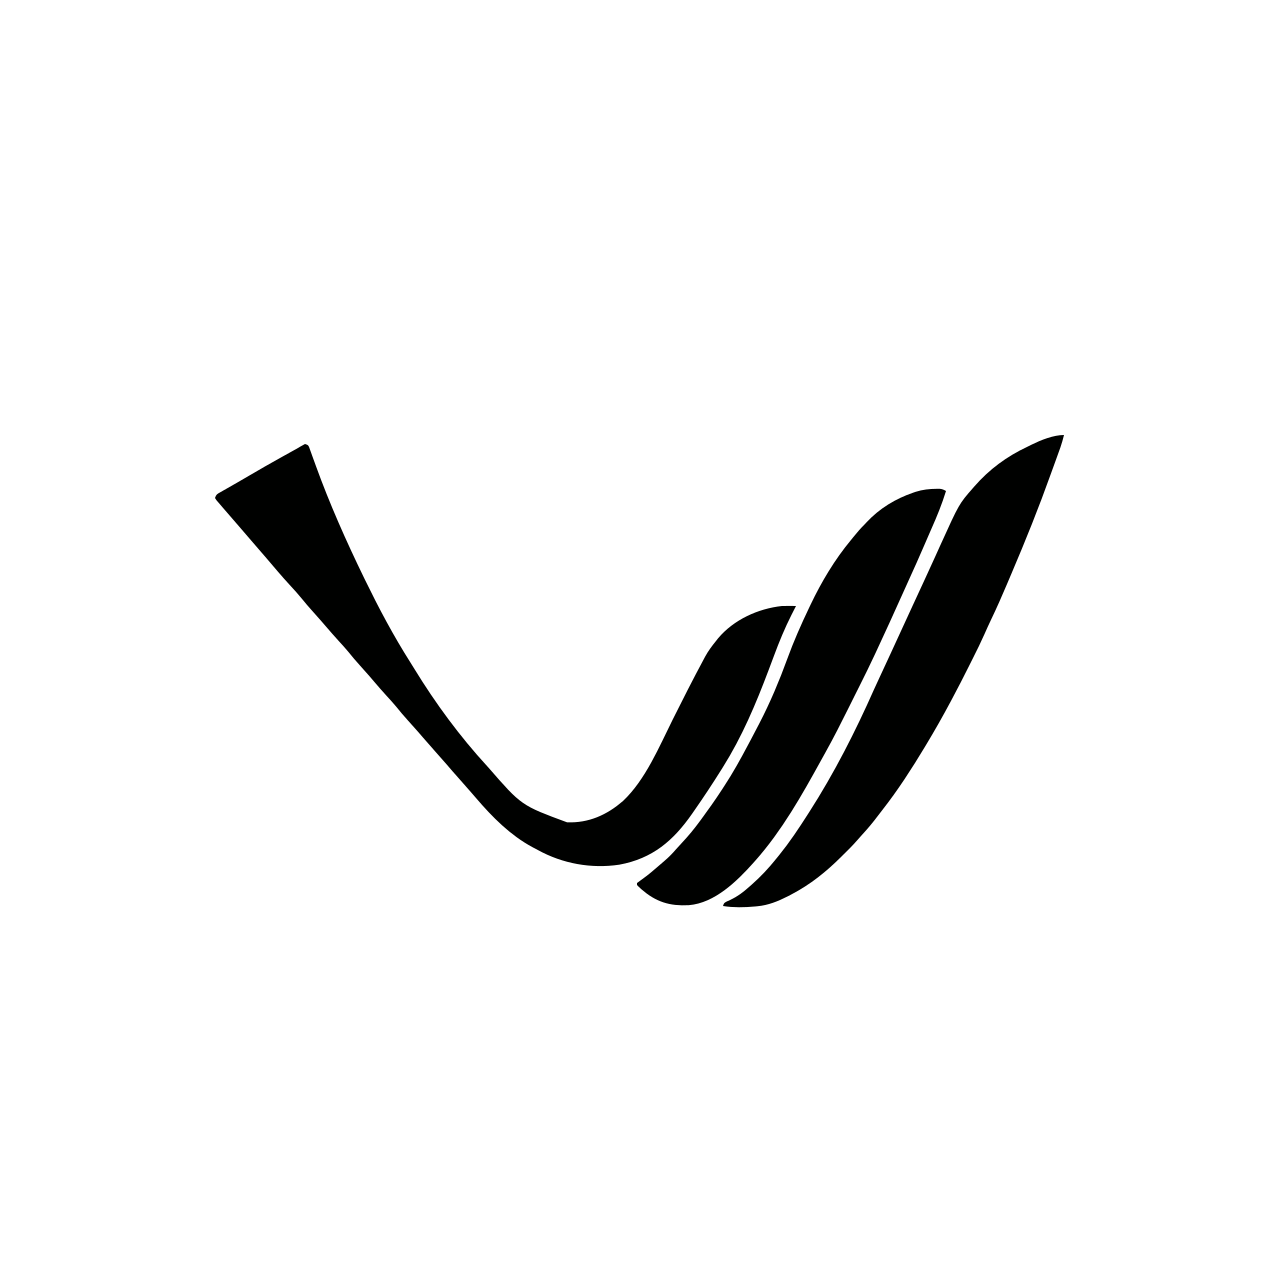
\includegraphics[width=2cm]{logo.png}
}

\begin{document}

\begin{frame}
\titlepage
\end{frame}

\begin{frame}[fragile]
\frametitle{About us}

\framesubtitle{}
\end{frame}

\begin{frame}[fragile]
\frametitle{Contents}

  \begin{enumerate}
    \item Chapter 1 - Motivations for our work
    \item Chapter 2 - Introduction to reconfigurable and heterogenouse computing
    \item Chapter 3 - Need for modern EDA compilers
    \item Chapter 4 - Work Done Towards Implementation  
  \end{enumerate}
\end{frame}

\begin{frame}[c,fragile]
  \frametitle{}
  \centering
  \textbf{Chapter 1}
  \centering
  Motivations for our work
\end{frame}

\begin{frame}[fragile]
\frametitle{Problems facing modern compute}
\framesubtitle{Moores law is slowing down}

  \begin{figure}
    \centering
    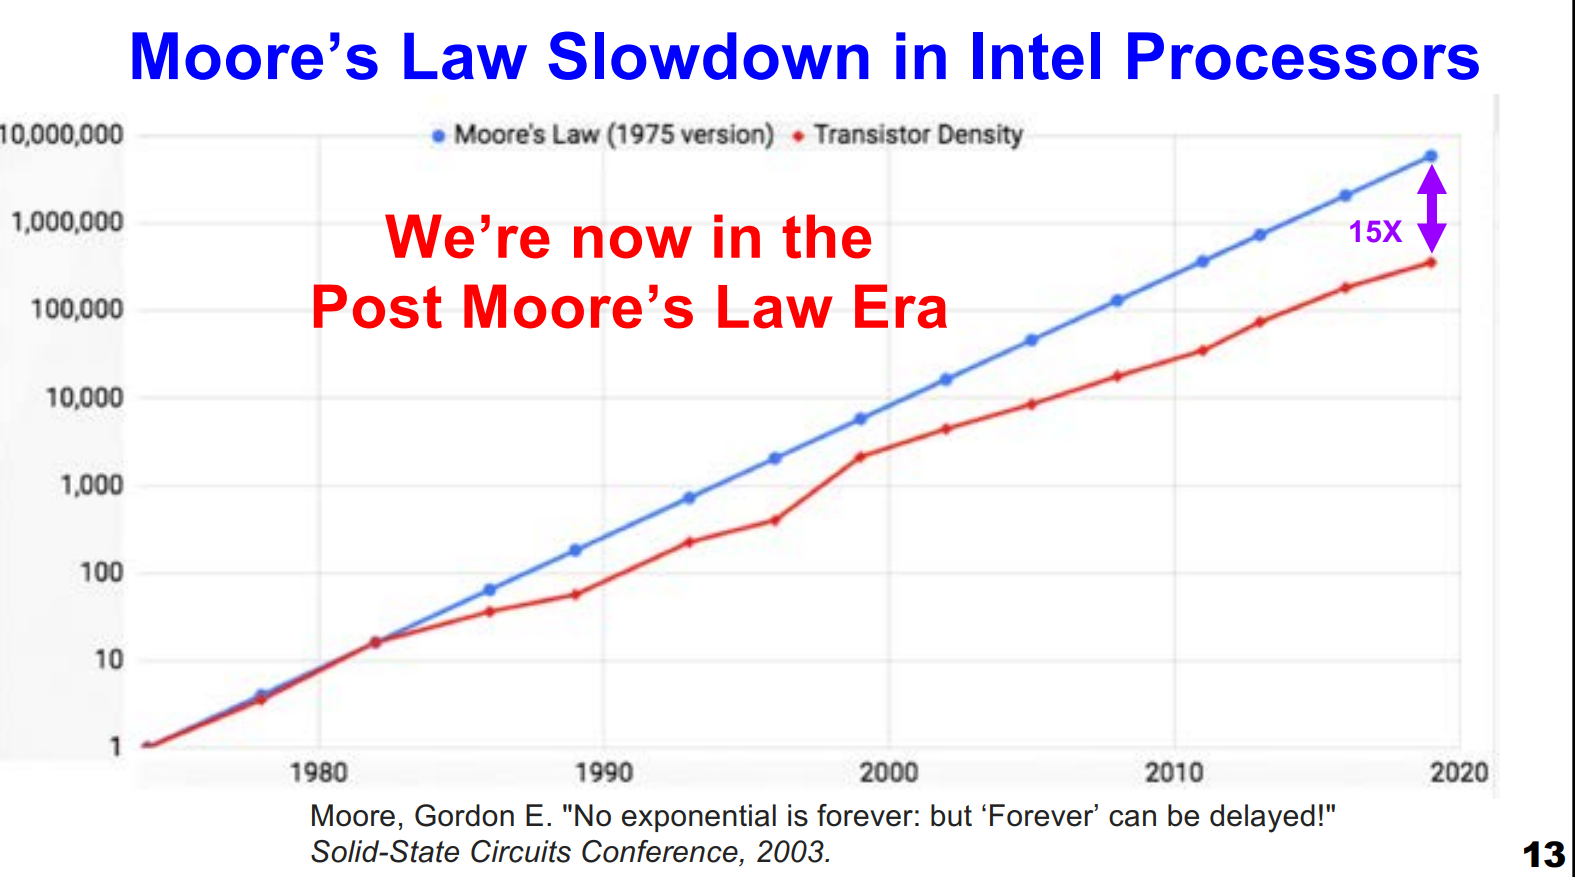
\includegraphics[width=0.85\textwidth]{mooreslaw.png}
    \caption{From "A Golden Age of Computers - David Patterson"}
  \end{figure}

\end{frame}

\begin{frame}[fragile]
\frametitle{Problems facing modern compute}
  \framesubtitle{Dennard Scaling has stopped working}

  \begin{figure}
    \centering
    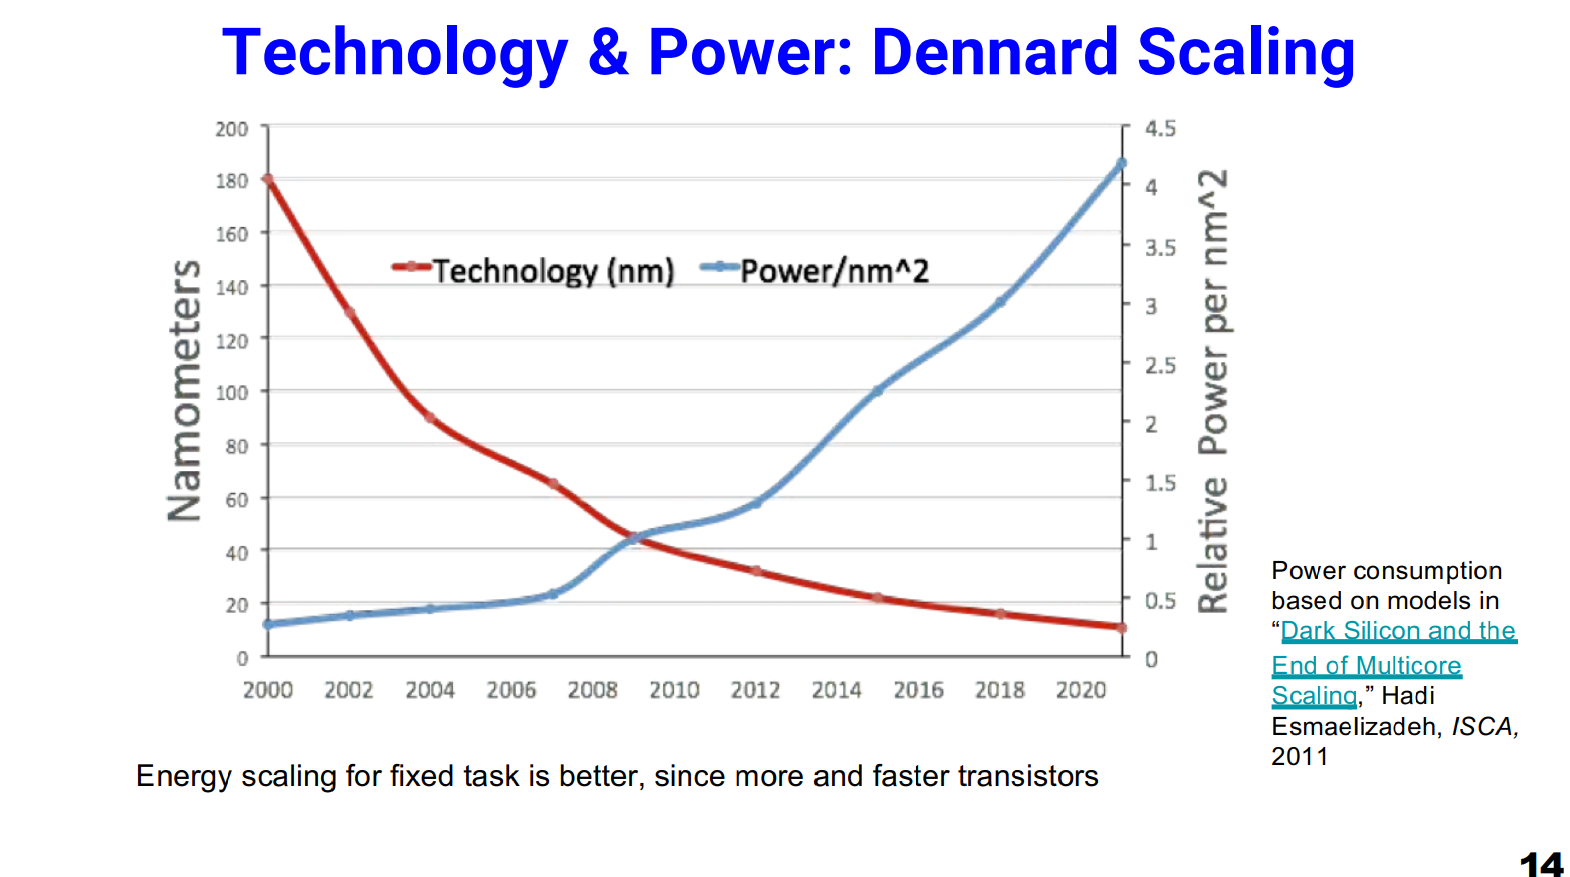
\includegraphics[width=0.85\textwidth]{dennardscaling.png}
    \caption{From "A Golden Age of Computers - David Patterson"}
  \end{figure}
\end{frame}

\begin{frame}[fragile]
\frametitle{Problems facing modern compute}
  \framesubtitle{}
  \begin{enumerate}
    \item The free lunch afforded by hardware improvements over years
      is coming to an end
    \item Hardwares are designed first and complying softwares to support
      them after it.
    \item New and creative architectures need to be designed along with the
      softwares abstractions to use them. 
  \end{enumerate}
\end{frame}


\begin{frame}[fragile]
\frametitle{Overview of Modern Compute}
\framesubtitle{}
  \begin{enumerate}
    \item An average motherboard has a CPU and optionally a GPU
    \item In specialized domains, one may find ASICs being used (for eg, 
      ML acceleration)
    \item ASICs are pretty cool (and fast) and solve domain specific problems
      that CPU/GPUs may not be able to solve, but are they for everyone?
    \item For starters, they are expensive to engineer and require a team
      of expert hardware engineers to be designed and fabricated
    \item Once that's done, expert systems software engineers are required
      to make the ASIC usable/compatible with the existing operating systems.
    \item A lot of hardwork, definitely not for everyone.  As a result, ASICs are far and few
    \item Should modern compute be restricted to CPUs/GPUs and a handful
      of ASICs?
    \item What about the problems where none of existing compute suffices?
  \end{enumerate}
\end{frame}

\begin{frame}[fragile]
  \frametitle{Hard-to-solve Problems for Modern Compute}
  \framesubtitle{Example 1}
  \textbf{Problems involving many peripherals as well as compute}

  For example, \\

  An embedded application that uses object detection to find
  objects in a line of sight and responds to it by driving many motors in
  real time needs heavy compute (for OD) and flexible IO to be able to 
  drive all the motors reliably. \\

  Existing solution would involve usign a GPU for ML workload, an
  driving the motors from a CPU. A CPU may or may not have as many IOs
  as required, in which case an IO expander may have to be set up.
\end{frame}

\begin{frame}[fragile]
  \frametitle{Hard-to-solve Problems for Modern Compute}
  \framesubtitle{Example 2}
  \textbf{Unusual Representation of Numbers}

  Quantization is a technique of reducing precision of numbers at the loss of
  accuracy. Quantization is used extensively to speed up Neural Network
  inference. New techniques such as heterogenous quantization of layers (i.e.
  different bit-widths of numbers at layer granularity), odd-number quantization
  (such as 9-bit numbers), ternary computers etc. pose a significant challenge
  for existing fixed-bit-width computers. 

\end{frame}

\begin{frame}[fragile]
  \frametitle{Hard-to-solve Problems for Modern Compute}
  \framesubtitle{Example 3}
  \textbf{New Architectures/Solutions for Old Problems}

  New solutions to old problems are those that are fundamentally different to
  all existing solutions. For example, Kolmogorov-Arnold Networks (KANs) propose
  an alternative to MLPs (which is at the core of machine learning today). KANs
  reeplace the static parameter of MLPs with a learnt spline function. Wrappers
  can be built around existing hardware to execute KANs too, but since its
  different on a fundamental level, dedicated hardwares would be beneficial.

\end{frame}

\begin{frame}[fragile]
  \frametitle{Hard-to-solve Problems for Modern Compute}
  \framesubtitle{Example 4}

  \textbf{Power-efficiency without sacrifices}

  Unlike general purpose chips, on FPGAs you only get what you need. As a
  result, the overall power efficiency of dedicated hardware tends to be
  higher than general purpose processors. 

  Customizable architecture eliminates unused components and reconfigurability
  allows adapting to changing workloads

\end{frame}

\begin{frame}[fragile]
  \frametitle{"Should I throw away my CPU?"}
  \framesubtitle{}
  \begin{enumerate}
    \item Strengths of existing compute are known. We would like
      to have these strengths in our systems and bring reconfigurable
      heterogenous compute to tackle the weaknesses. 
    \item We don't have to forego our CPUs, GPUs.
    \item CPUs are good at running operating systems, they should continue
      doing it. 
    \item The goal is to \textcolor{green}{complement} existing compute not
      \textcolor{red}{replace}.
  \end{enumerate}

\end{frame}

\begin{frame}[c,fragile]
  \frametitle{}

  \centering
  \textbf{Chapter 2}
  \centering
  Introduction To Reconfigurable And Heterogenous Computing
\end{frame}

\begin{frame}[fragile]
  \frametitle{Setting the stage}
  \framesubtitle{}
    Two key ideas:
      \begin{enumerate}
        \item Reconfiguration: The process through which a "reconfigurable
      processor" is re-programmed to implement a new circuit
        \item Heterogeneity: A system must include processors of different 
          capacities/abilites well integrated together.
      \end{enumerate}
\end{frame}

\begin{frame}[fragile]
\frametitle{Reconfigurability: An Introduction to FPGAs}
\framesubtitle{}
  \begin{enumerate}
    \item FPGAs are a grid of cells that can be reprogrammed to implement
      any circuit. 
    \item Digital circuits consist of gates (that implement logic) and
      connections (that connect gates to each other).
    \item FPGAs, at the core, consist of SRAM cells (that implement the
      functionality of gates by storing their truth-tables in SRAM cells) and
      programmable interconnect (implemented via switch boxes) that allow
      connections
    \item Circuits for FPGAs are described using Hardware Descriptions Languages
      (HDLs) such as Verilog, VHDL.
    \item High level description of a circuit is compiled into real hardware
      (i.e. a representation that only uses FPGA primitives) by a "compiler"
  \end{enumerate}

\end{frame}

\begin{frame}[fragile]
\frametitle{Key problems with reconfigurable-heterogenous computing}
\framesubtitle{}
  \begin{enumerate}
    \item To implement a reconfigurable heterogenous computer with FPGAs,
      the problems are two-fold:
    \item Problem 1: Using FPGAs with traditional softwares are in-convenient.
    \item Problem 2: Writing new hardwares for FPGAs, implementing custom solutions is
      tedious with a very steep learning curve, often times requiring 
      domain expertise.
  \end{enumerate}
\end{frame}

\begin{frame}[fragile]
\frametitle{Problem 1: Programming model for FPGAs}
\framesubtitle{}
  \begin{enumerate}
    \item GPUs enjoy a concrete and abstract programming model
    \item No true industry grade programming model exists for FPGAs
    \item There's OpenCL support for FPGAs. But that involves treating
      FPGAs like an ASIC.
    \item A true programming model for FPGAs would heavily exploit
      reconfigurability
  \end{enumerate}
\end{frame}

\begin{frame}[fragile]
  \frametitle{Comparison of a reconfigurable-heterogenous programming model with a von-neumann
  computer}
  \framesubtitle{}
  \begin{figure}
    \centering
    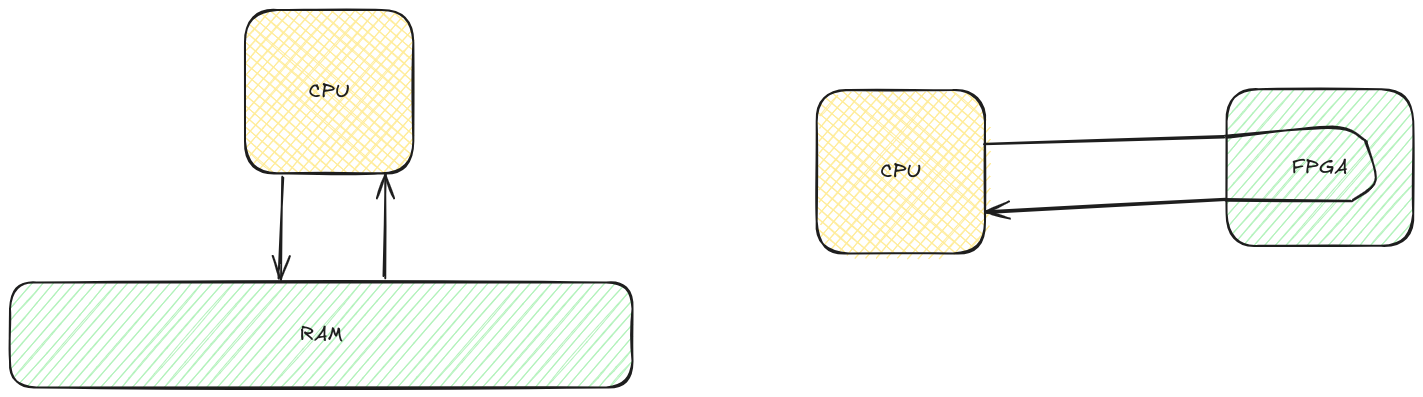
\includegraphics[width=0.75\textwidth]{flow.png}
    \caption{a) A von-neumann computer b) a flowing reconfigurable computer}
    \label{}
  \end{figure}
  Figure a) shows the difference b/w a von-neuman computer (which executes
  \textbf{instructions} on \textbf{data} over a \textbf{bus} resulting in
  back-and-forth of computation. 

  Figure b) is a flow computer where the
  hardware is configured to cause incoming data to be transformed in the
  way desired. There are \textcolor{red}{no instructions} as the hardware
  is configured to a desired operation. Data flows in and out
  of the chip transformed. 
\end{frame}

\begin{frame}[fragile]
  \frametitle{Comparison of a reconfigurable-heterogenous programming model with a von-neumann
  computer}
  \framesubtitle{}
  It could be said from the previous slide that the reconfigurable style of
  architecture has no Instruction Set Architecture (ISA) (hence the title
  of this talk). "What to do with data" is a part of the hardware, instead
  of being attached with the data in the form of instructions. It's the
  only thing that it does.
  Following are a few examples of reconfigurable no-ISA architecture. They
  include a JPEG encoder and a CNN accelerator:
\end{frame}



\begin{frame}[fragile]
  \frametitle{Flow architecture for JPEG encoding}
  \framesubtitle{}
  \begin{figure}
    \centering
    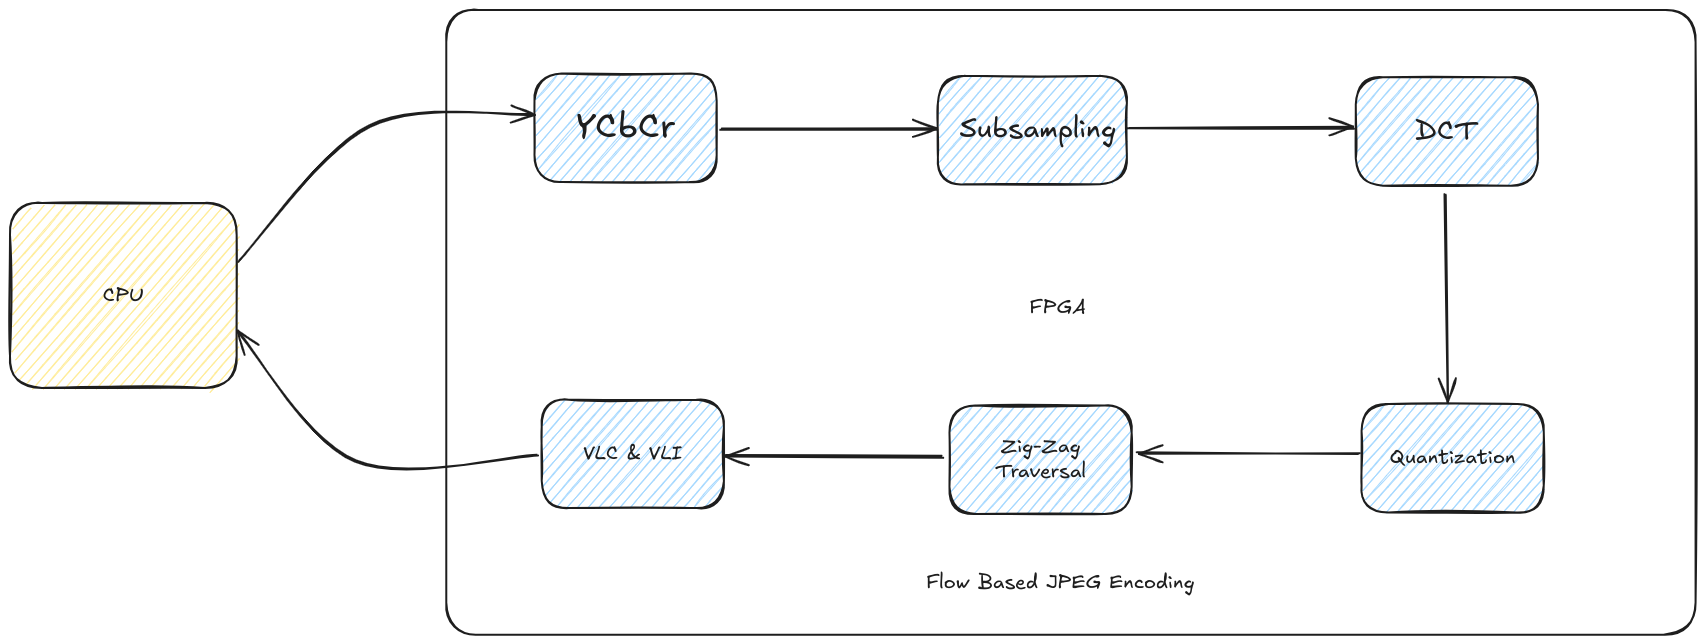
\includegraphics[width=0.95\textwidth]{flowjpeg.png}
    \caption{JPEG compression. Each operation has its own hardware}
    \label{}
  \end{figure}

  RAW images flow in, pass through the blocks, being encoded
  and the process and JPEG compressed images come out
\end{frame}

\begin{frame}[fragile]
  \frametitle{Flow architecture for CNN inference}
  \framesubtitle{}
  \begin{figure}
    \centering
    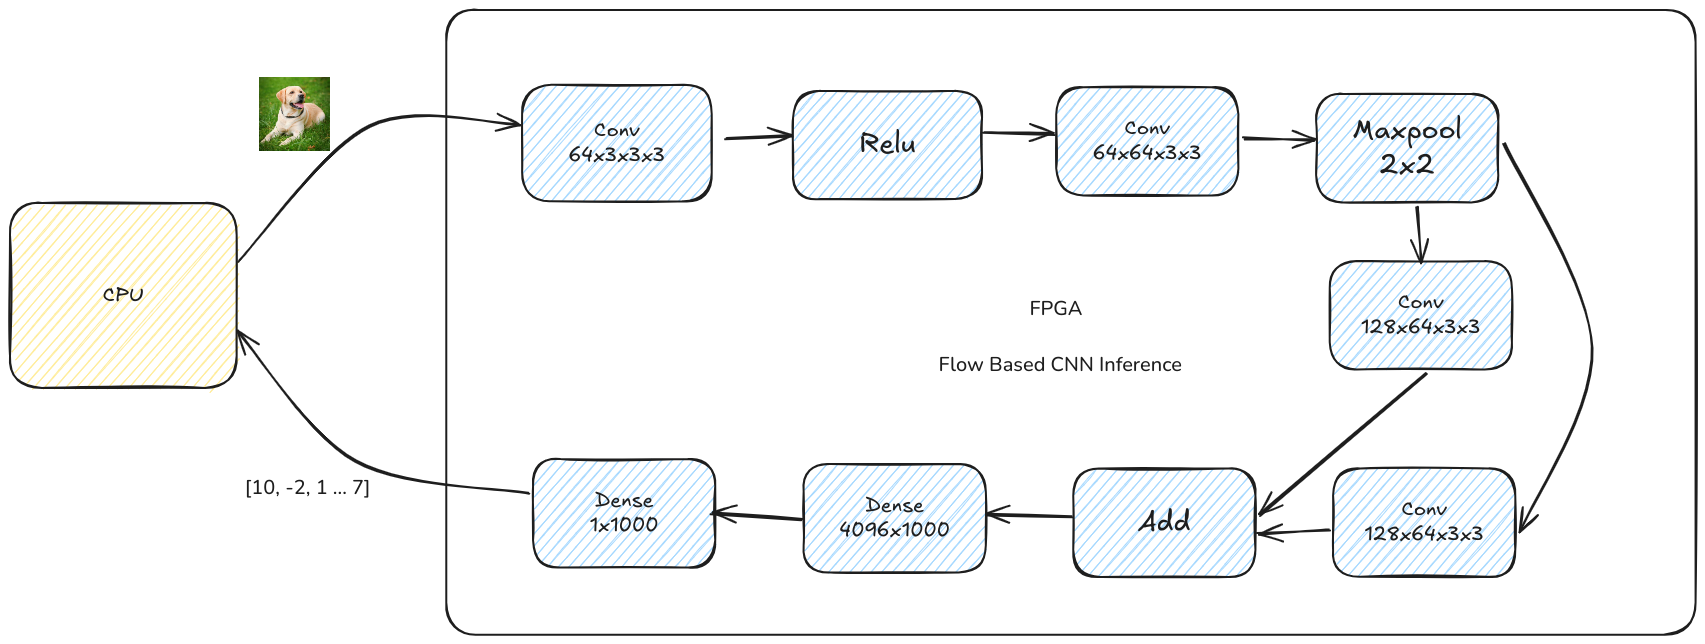
\includegraphics[width=0.95\textwidth]{flowcnn.png}
    \caption{CNN inference. Each layer of a network has its own hardware}
    \label{}
  \end{figure}

  Images (according to the pre-process pipeline of a network) flow
  in, each layer manipulates and passes its computation to the
  hardware after it and end-results are returned by the last
  block.
\end{frame}

\begin{frame}[fragile]
  \frametitle{Observation on flow-based computers}
  \framesubtitle{}
  \begin{enumerate}
      
    \item Hardwares for a problem are generated by a "Compiler" from a high-level
      specification that describes connection of coarse functions.
    \item Any coarse hardware can be programatically be plucked and placed in a
      different setting thanks to the compilers ability to reason with hardware
      connections.
    \item Flow based computer exibit a more functional approach towards
      computation
    \item On a coarser scale, purity of computation is maintained as hardware
      blocks do not depend on a global state to execute
  \end{enumerate}
\end{frame}

\begin{frame}[fragile]
  \frametitle{An exemplary DSL for reconfigurable compute architectures}
\framesubtitle{}
  Following is an example of a DSL that allows specification of coarse hardware.
  It provides an interface to define connections b/w hardware, control
  reconfiguration (through existing programming constructs (slide 3) and
  integrate it with existing codebases

\end{frame}

\begin{frame}[fragile]
  \frametitle{An exemplary DSL for reconfigurable compute architectures}
\framesubtitle{}
  \begin{verbatim}
    Base *input = new Tensor(std::vector<int>{1,2,3,4}, 
                    "t1");
    Base *b = new MLEngineCore(input, "gc1");
    *b = input;
    Base *b1 = new PeripheralMultiplex(b, "AHB", "pp1");
    *b1 = b;
    for (int i = 0; i < 100; ++i) {
    Base *b1 = new Sha256(b);
    *b1 = b;
    }
    Model m1 = new Model(input, b1);
  \end{verbatim}

  Describes an Mlaccelerator connected to a peripheral multiplexor
  which is connected to 100 Sha256 blocks, all through c++.
\end{frame}

\begin{frame}[fragile]
  \frametitle{An exemplary DSL for reconfigurable compute architectures (2)}
\framesubtitle{}
  \begin{verbatim}
    Base *cam_in = new CameraCore("MIPI0", "cam1");
    Base *proc_one = new GaussianBlurCore(input, "gc1");
    *proc_one = cam_in;
    Base *display_out = new 
        PeripheralMultiplex(b, "LVDS", "pp1");
    *display_out = proc_one;
    Model m2 = new Model(cam_in, display_out);
  \end{verbatim}
  Describes an application that takes input from camera,
  implements gaussian blur on it and returns it to an LVDS interface on the
  FPGA.

\end{frame}

\begin{frame}[fragile]
  \frametitle{An exemplary DSL for reconfigurable compute architectures (3)}
\framesubtitle{}
  \begin{verbatim}
    m1->compute(input);
    if (some_user_defined_condition(m1->output())) {
      m2->compute(m1->output());
    } else {
      return m1->out();
    }
\end{verbatim}
  \texttt{model->compute} is the function that triggers generation, flashing and
  computation on a hardware described by a Model.

  Demonstrates conditional reconfiguration where based on \texttt{m1->compute}'s
  result. If the result meets a user specified condition, m2's hardware is
  generated, flashed and computation begins for it.
\end{frame}

\begin{frame}[c,fragile]
  \frametitle{}

  \centering
  \textbf{Chapter 3} 
  \centering
  Need for modern EDA compilers
\end{frame}

\begin{frame}[fragile]
  \frametitle{Problem 2: Writing hardwares is hard}
  \framesubtitle{}
  \begin{enumerate}
    \item Writing HDLs is a tedious task often requiring domain expertise
    \item EDA tools are propreitary and hard-to-work-with
    \item The general problem of compilation of hardwares is NP-Complete but
      there are special cases that can be exploited.
  \end{enumerate}
\end{frame}


\begin{frame}[fragile]
  \frametitle{Opensource EDA Compilers}
  \framesubtitle{}
  \begin{enumerate}
    \item Groups such as f4pga, YosysHQ, openfpga are trying to create opensource
      alternatives for proprietary CAD tools by reverse engineering FPGAs
      but are limited by the resources 
    \item Creating Open Software infrastructure for Hardware (flexibility),
      which is community driven 
    \item Most of the opensource EDA compilers such as Yosys, CIRCT, Verilator,
      openvaf can't create real hardware. They are limited to
      logical synthesis and simulation.
  \end{enumerate}

\end{frame}

\newcommand\myheading[1]{%
  \par\bigskip
  {\Large\bfseries#1}\par\smallskip}

\begin{frame}[fragile]
    \frametitle{Compilers in EDA}
     \myheading{Yosys} 
        \begin{enumerate}
            \item Compiler that generates  verilog to netlist format(support Technology mapping)
            \item IR : RTLIL
            \item SupportSimulation: CXXRTL (cycle driven simulator)(supports only 2 states
            \item Largely community Driven
        \end{enumerate}
    \myheading{Verilator}
        \begin{enumerate}
            \item Compiler that generates Cpp code from Verilog files
            \item Used Extensively for cycle based simualation (supports only 2 states )
            \item competes with proprietary simulators ,Community Driven
        \end{enumerate}
    
\end{frame}

\begin{frame}[fragile]
    \frametitle{Compilers in EDA}
    \myheading{CIRCT}
        \begin{enumerate}
            \item Modular usage of libraries, designs similar to LLVM/MLIR in Hardware  
            \item \{HLS,sv\} to \{sv,vcd etc ... \}
            \item Hardware MLIR  Dialects 
            \item Arcilator used for simulation 
                \item cycle based simualation (supports only 2 states )
            \item Supports only simulation 
        \end{enumerate}
    \myheading{Openvaf}
        \begin{enumerate}
            \item Verilog-A frontend 
            \item uses LLVM and generates a binary file for simulation
        \end{enumerate}
\end{frame}


\begin{frame}[fragile]
  \frametitle{FPGA CAD Toolflow}
  \framesubtitle{}
   \begin{figure}
        \centering
        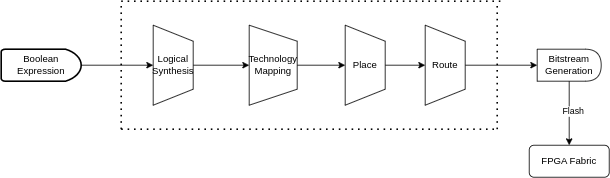
\includegraphics[width=1\linewidth]{images/cad_flow_fl.png}
        \caption{FPGA CAD Tool Flow }
        \label{exa_cadflow}
    \end{figure}
   
\end{frame}

\begin{frame}[fragile]
    \frametitle{FPGA CAD Toolflow: The Frontend}
    \framesubtitle{Logical Synthesis,Technology Mapping}
    \begin{enumerate}
      \item Logical synthesis is the process that parses HDL, performs
        technology-agnostic optimizations, and outputs a circuit (netlist)
        of generic primitives
      \item Technology Mapping maps generic primitives generated by synthesis to
        FPGA-specific primitives. 
    \end{enumerate}
    \begin{figure}
        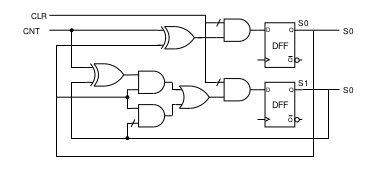
\includegraphics[width=0.5\linewidth]{images/netlist_gate.png}
        \caption{Gates Mapped for given Expression}
        \label{exa_mapgate}
    \end{figure}

\end{frame}

\begin{frame}[fragile]
  \frametitle{FPGA CAD Toolflow: Synthesis/Mapping Via Example}
  boolean expression:
   \[{S}_0 = \overline{CNT}\cdot{S}_0+ CNT \cdot \overline{{S}_0} \]
   \[{S}_1  ={S}_1 (\overline{CNT} \cdot\overline{{S}_0}) + CNT\cdot{S}_0\cdot\overline{{S}_1} \]
    \begin{figure}[h]
        \begin{subfigure}{.5\textwidth}
            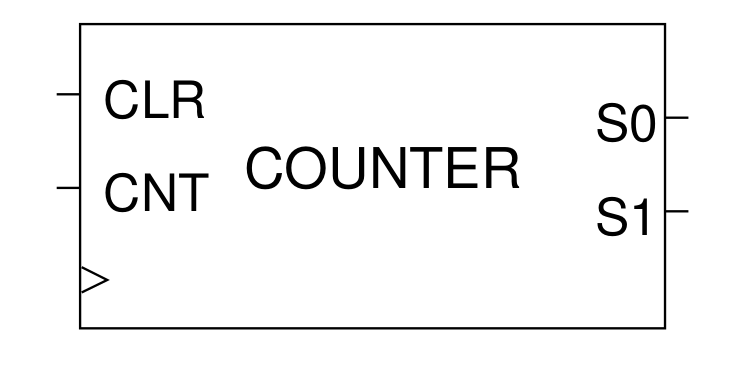
\includegraphics[width=0.9\linewidth]{slides/images/basic_block.png} 
             \caption{Two bit counter block}
             \label{fig:subim1}
        \end{subfigure}
        \begin{subfigure}{.5\textwidth}
             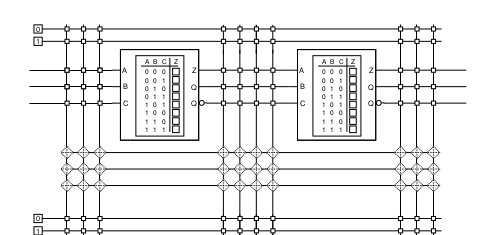
\includegraphics[width=0.9\linewidth]{slides/images/LUT.png}
             \caption{Example LUT }
             \label{fig:subim2}
             \end{subfigure}
    \end{figure}
\end{frame}



\begin{frame}[fragile]
  \frametitle{FPGA CAD Toolflow: The Backend}
  \framesubtitle{Placement}
  \begin{figure}
    \centering
    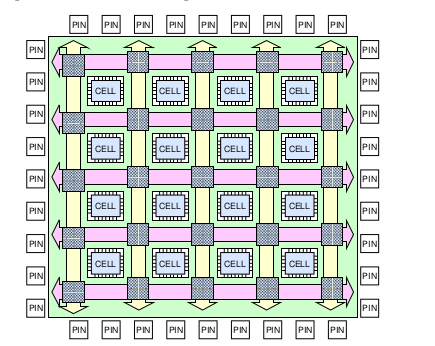
\includegraphics[width=0.5\linewidth]{images/FPGA_Fabric.png}
    \caption{Example FPGA Fabric}
    \label{exa-fabric}
  \end{figure}

  Simulated Annealing (industry standard Algorithm) to place based on Minimum cost model 
\end{frame}

\begin{frame}[fragile]
  \frametitle{FPGA CAD Toolflow: The Backend}
  \framesubtitle{Routing}
  Routing : interconnect the Configurable Logic  blocks with minimum timing cost 
  \begin{figure}
    \centering
    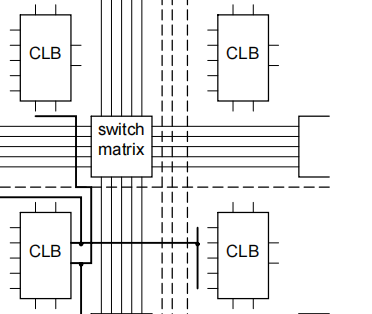
\includegraphics[width=0.5\linewidth]{images/switch_matrix.png}
    \caption{FPGA Interconnect }
    \label{exa_interconnect}
  \end{figure}
\end{frame}

\begin{frame}[fragile]
  \frametitle{FPGA CAD Toolflow: Backend via Example}
  \framesubtitle{Placement, Routing}

  Placement and Routing for Two Bit counter would be 

  \begin{figure}
    \centering
    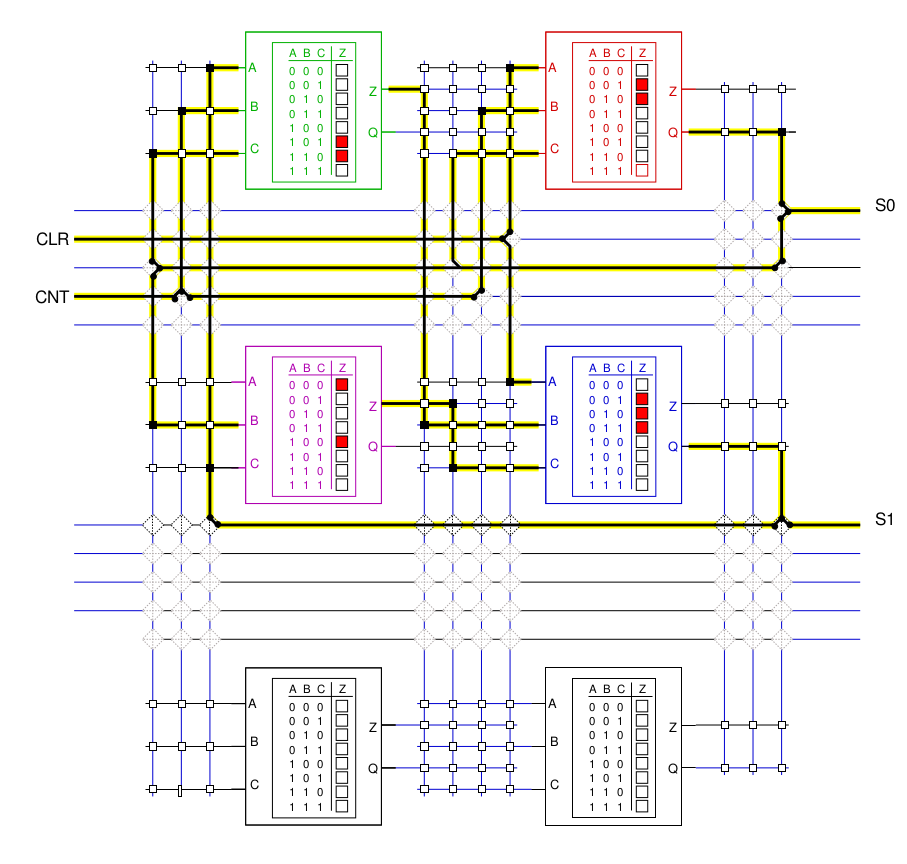
\includegraphics[width=0.5\linewidth]{images/fpga_luts.png}
    \caption{LUTs Connected with wire  }
    \label{exa_interconnect}
  \end{figure}
  **todo Add Image credits and make images more consise 
  Add opensource compilation process 
\end{frame}

\begin{frame}[fragile]
  \frametitle{Optimization oppurtunity for EDA compilers}
  \framesubtitle{}
  \begin{enumerate}
    \item Our DSL compiler connects hardwares together. The mapping phase
      of hardware generation can be completely by-passed if the compiler can
      be designed to operate on netlists directly instead of verilog.
    \item Mapping process involves among many steps a phase where it looks
      for a minimal boolean expression. In iterative write-compile-debug loops
      entire hardware may not change frequently so their resulting minimal
      boolean expressions can be cached and further sped up by performing a
      look up in this cache instead of searching all over again.
    \item Routing can be designed to make use of GPUs 
  \end{enumerate}
\end{frame}

\begin{frame}[c,fragile]

  \centering
  \textbf{Chapter 4}
  Work Done Towards Implementation
\end{frame}

\begin{frame}[fragile]
  \frametitle{Realizing this goal}
  \begin{enumerate}
    \item Realizing this goal requires designing and implementation from
      first principles
    \item To achieve this, we designed our own hardware: Vaaman
    \item To understand the nature of applications (in the sense of what
      bottlenecks exist and whether or not a certain application would
      benefit from reconfigurable-heterogenous architecture), projects have been implemented
    \item These include: Gati (an ML accelerator) and Periplex (a peripheral
      multiplexor)
    \item Discussion on this work follows:
  \end{enumerate}
  \framesubtitle{}
\end{frame}

\begin{frame}[fragile]
  \frametitle{The Hardware (Vaaman)}
  \framesubtitle{}
  \begin{figure}
    \centering
    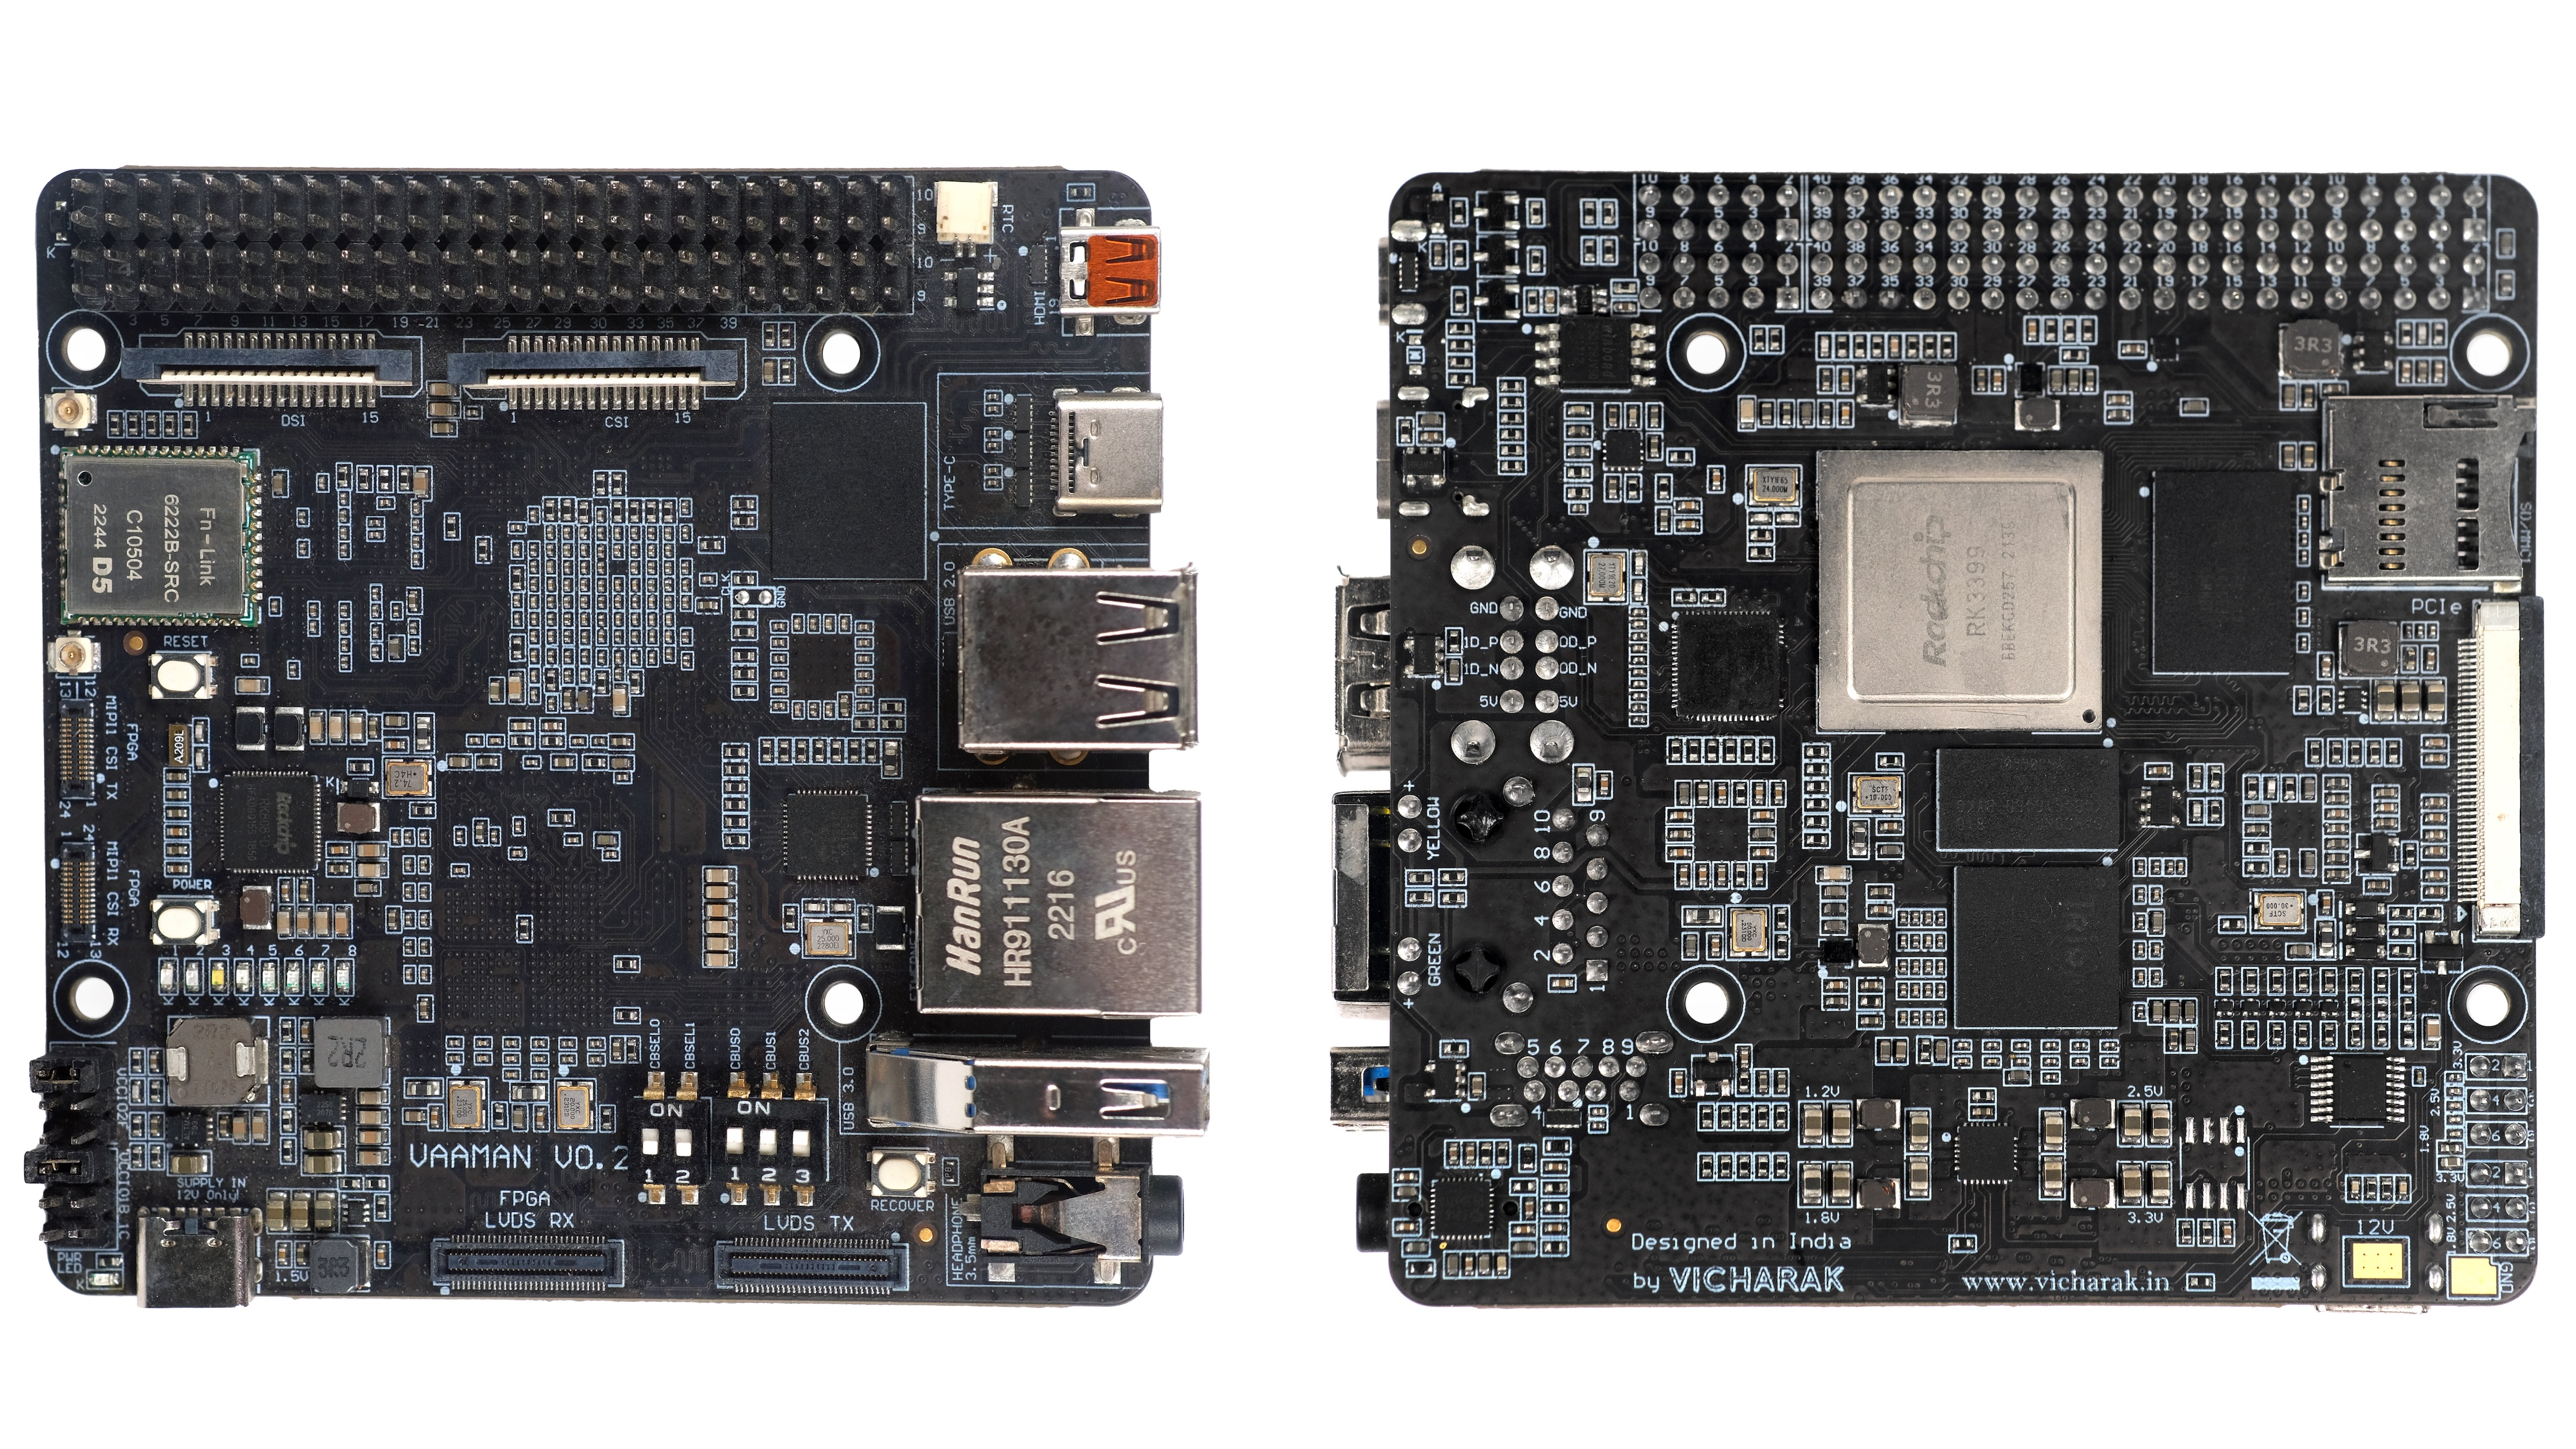
\includegraphics[width=0.95\textwidth]{vaaman.jpg}
    \caption{Vaaman: A heterogenous SBC}
    \label{neuron}
  \end{figure}
\end{frame}

\begin{frame}[fragile]
  \frametitle{Implementation: ML Accelerator (Gati)}
  Gati is a set of hardware and software programs that perform CNN
  acceleration with FPGA as a co-processor.
  \begin{enumerate}
    \item At the core of gati is a systolic array pipeline based MAC engine
    \item The Gati-ISA is macro (i.e. implements complex operations directly
      like Convolution) instead of breaking them down into primitives
    \item The instructions have almost a one-to-one match with 'layers'
      from a neural network
    \item Assisting this hardware is a Compiler/Runtime.
    \item The compiler does two primary things:
      \begin{enumerate}
        \item Parsing of input data and NN models (protobufs etc.),
          transpositions of kernels to allow contiguos memory access, and generation
          of a byte stream that can be fed to the FPGA
        \item Generating custom hardware for every nn model
      \end{enumerate}
    \item The runtime partitions a network into execute-on-host and
      execute-on-device, re-orders inputs, and offloads computation
      to the FPGA
  \end{enumerate}
\end{frame}

\begin{frame}[fragile]
  \frametitle{Gati has an ISA? But you said ISAs are bad?}
  Gati is a testbed for modelling complex problems found in real world.
  At the moment it does and doesn not do many things that we eventually want
  from it.
  For example:
  \begin{enumerate}
    \item Gati has a hardware generator. If this generator is generalized
      enouugh, we end up solving a part of problem 1.
    \item It still uses an ISA. But its possible to partition an ML
      model so that it can entirely fit into 
      the FPGA hardwired to do only a part of the model followed by
      reconfiguration to execute later parts.
  \end{enumerate}
\end{frame}

\begin{frame}[fragile]
  \frametitle{Implementation: Peripheral Multiplexor (Periplex)}
  \framesubtitle{}

  \begin{enumerate}
    \item Periplex is a interface translator that allows communication
      between a set of inputs from a set of protocols to a set of outputs
      in another set of protocols
    \item Consider, an application where 2 inputs each from an SPI bus and an
      I2C bus need to drive 2 motors whose controller speaks CAN. Periplex can
      be used to easily make hardware and enable this communication.
    \item Periplex is, in a sense, the swiss army knife of embedded
      communication protocols.
  \end{enumerate}
\end{frame}

\begin{frame}[fragile]
  \frametitle{Conclusion}
  \framesubtitle{}

  \begin{enumerate}
    \item Reconfigurable architectures can provide a way to solve many problems
      that existing compute struggle with
    \item Reconfigurable architectures as demostrated previously can help
      alleviate von-neumann bottleneck.
  \end{enumerate}
\end{frame}

\end{document}
